\chapter{Computer Graphics Primer}
\label{chap:cgp}

\firstletter{C}omputer graphics is the foundation of data visualization. Practically speaking, visualization is the process that transforms data into a set of graphics primitives. The methods of computer graphics are then used to convert these primitives into pictures or animations. This chapter discusses basic computer graphics principles. We begin by describing how lights and physical objects interact to form what we see. Next we examine how to simulate these interactions using computer graphics techniques. Hardware issues play an important role here since modern computers have built-in hardware support for graphics. The chapter concludes with a series of examples that illustrate our object-oriented model for 3D computer graphics.

\section{Introduction}

Computer graphics is the process of generating images using computers. We call this process \emph{rendering}. There are many types of rendering processes, ranging from 2D paint programs to sophisticated 3D techniques. In this chapter we focus on basic 3D techniques for visualization.

We can view rendering as the process of converting graphical data into an image. In data visualization our goal is to transform data into graphical data, or \emph{graphics primitives}, that are then rendered. The goal of our rendering is not so much photo realism as it is information content. We also strive for interactive graphical displays with which it is possible to directly manipulate the underlying data. This chapter explains the process of rendering an image from graphical data. We begin by looking at the way lights, cameras, and objects (or actors) interact in the world around us. From this foundation we explain how to simulate this process on a computer.

\section{A Physical Description of Rendering}

\begin{figure}[ht]
  \centering
  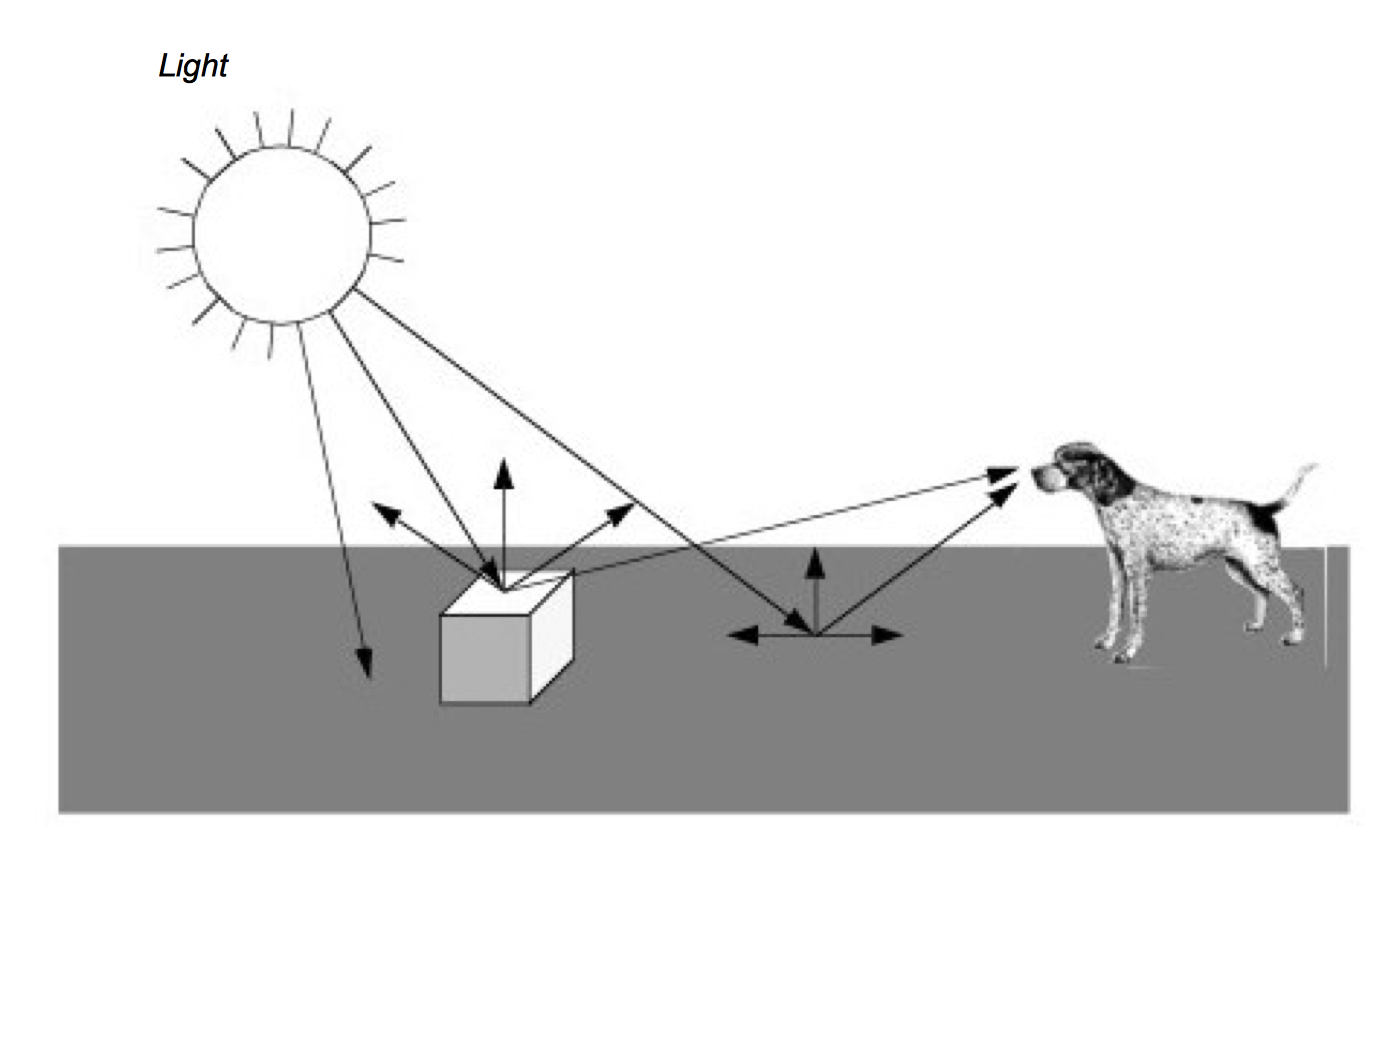
\includegraphics[width=0.8\textwidth]{Figure3-1}\\
  \caption{Physical generation of an image.}\label{fig:Figure3-1}
\end{figure}

Figure \ref{fig:Figure3-1} presents a simplified view of what happens when we look at an object, in this case a cube. Rays of light are emitted from a light source in all directions. (In this example we assume that the light source is the sun.) Some of these rays happen to strike the cube whose surface absorbs some of the incident light and reflects the rest of it. Some of this reflected light may head towards us and enter our eyes. If this happens, then we "see" the object. Likewise, some of the light from the sun will strike the ground and some small percentage of it will be reflected into our eyes.

As you can imagine, the chances of a ray of light travelling from the sun through space to hit a small object on a relatively small planet are low. This is compounded by the slim odds that the ray of light will reflect off the object and into our eyes. The only reason we can see is that the sun produces such an enormous amount of light that it overwhelms the odds. While this may work in real life, trying to simulate it with a computer can be difficult. Fortunately, there are other ways to look at this problem.

A common and effective technique for 3D computer graphics is called \emph{ray-tracing} or \emph{ray-casting}. Ray-tracing simulates the interaction of light with objects by following the path of each light ray. Typically, we follow the ray backwards from the viewer's eyes and into the world to determine what the ray strikes. The direction of the ray is in the direction we are looking (i.e., the view direction) including effects of perspective (if desired). When a ray intersects an object, we can determine if that point is being lit by our light source. This is done by tracing a ray from the point of intersection towards the light. If the ray intersects the light, then the point is being lit. If the ray intersects something else before it gets to the light, then that light will not contribute to illuminating the point. For multiple light sources we just repeat this process for each light source. The total contributions from all the light sources, plus any ambient scattered light, will determine the total lighting or shadow for that point. By following the light's path backwards, ray tracing only looks at rays that end up entering the viewer's eyes. This dramatically reduces the number of rays that must be computed by a simulation program.

Having described ray tracing as a rendering process, it may be surprising that many members of the graphics community do not use it. This is because ray tracing is a relatively slow image generation method since it is typically implemented in software. Other graphics techniques have been developed that generate images using dedicated computer hardware. To understand why this situation has emerged, it is instructive to briefly examine the taxonomy and history of computer graphics.

\subsection{Image-Order and Object-Order Methods}

Rendering processes can be broken into two categories: \emph{image-order} and \emph{object-order}. Ray tracing is an image-order process. It works by determining what happens to each ray of light, one at a time. An object-order process works by rendering each object, one at a time. In the above example, an object-order technique would proceed by first rendering the ground and then the cube.

To look at it another way consider painting a picture of a barn. Using an image-order algorithm you would start at the upper left corner of the canvas and put down a drop of the correct color paint. (Each paint drop is called a picture element or \emph{pixel}.) Then you would move a little to the right and put down another drop of paint. You would continue until you reached the right edge of the canvas, then you would move down a little and start on the next row. Each time you put down a drop of paint you make certain it is the correct color for each pixel on the canvas. When you are done you will have a painting of a barn.

An alternative approach is based on the more natural (at least for many people) object-order process. We work by painting the different objects in our scene, independent of where the objects actually are located on the scene. We may paint from back to front, front-to-back, or in arbitrary order. For example, we could start by painting the sky and then add in the ground. After these two objects were painted we would then add in the barn. In the image-order process we worked on the canvas in a very orderly fashion; left to right, top to bottom. With an object-order process we tend to jump from one part of the canvas to another, depending on what object we are drawing.

The field of computer graphics started out using object-order processes. Much of the early work was closely tied to the hardware display device, initially a vector display. This was little more than an oscilloscope, but it encouraged graphical data to be drawn as a series of line segments. As the original vector displays gave way to the currently ubiquitous raster displays, the notion of representing graphical data as a series of objects to be drawn was preserved. Much of the early work pioneered by Bresenham \cite{Bresenham65} at IBM focused on how to properly convert line segments into a form that would be suitable for line plotters. The same work was applied to the task of rendering lines onto the raster displays that replaced the oscilloscope. Since then the hardware has become more powerful and capable of displaying much more complex primitives than lines.

It wasn't until the early 1980s that a paper by Turner Whitted \cite{Whitted80} prompted many people to look at rendering from a more physical perspective. Eventually ray tracing became a serious competitor to the traditional object-order rendering techniques, due in part to the highly realistic images it can produce. Object-order rendering has maintained its popularity because there is a wealth of graphics hardware designed to quickly render objects. Ray tracing tends to be done without any specialized hardware and therefore is a time-consuming process.

\subsection{Surface versus Volume Rendering}

The discussion to this point in the text has tacitly assumed that when we render an object, we are viewing the surfaces of objects and their interactions with light. However, common objects such as clouds, water, and fog, are translucent, or scatter light that passes through them. Such objects cannot be rendered using a model based exclusively on surface interactions. Instead, we need to consider the changing properties inside the object to properly render them. We refer to these two rendering models as \emph{surface rendering} (i.e., render the surfaces of an object) and \emph{volume rendering} (i.e., render the surface and interior of an object).

Generally speaking, when we render an object using surface rendering techniques, we mathematically model the object with a surface description such as points, lines, triangles, polygons, or 2D and 3D splines. The interior of the object is not described, or only implicitly represented from the surface representation (i.e., surface is the boundary of the volume). Although techniques do exist that allow us to make the surface transparent or translucent, there are still many phenomena that cannot be simulated using surface rendering techniques alone (e.g., scattering or light emission). This is particularly true if we are trying to render data interior to an object, such as X-ray intensity from a CT scan.

Volume rendering techniques allow us to see the inhomogeneity inside objects. In the prior CT example, we can realistically reproduce X-ray images by considering the intensity values from both the surface and interior of the data. Although it is premature to describe this process at this point in the text, you can imagine extending our ray tracing example from the previous section. Thus rays not only interact with the surface of an object, they also interact with the interior.

In this chapter we focus on surface rendering techniques. While not as powerful as volume rendering, surface rendering is widely used because it is relatively fast compared to volumetric techniques, and allows us to create images for a wide variety of data and objects. Chapter 7 describes volume rendering in more detail.

\subsection{Visualization Not Graphics}

Although the authors would enjoy providing a thorough treatise on computer graphics, such a discourse is beyond the scope of this text. Instead we make the distinction between visualization (exploring, transforming, and mapping data) and computer graphics (mapping and rendering). The focus will be on the principles and practice of visualization, and not on 3D computer graphics. In this chapter and Chapter 7 we introduce basic concepts and provide a working knowledge of 3D computer graphics. For those more interested in this field, we refer you to the texts recommended in the "Bibliographic Notes" on page \pageref{Ch03BibNotes} at the end of this chapter.

One of the regrets we have regarding this posture is that certain rendering techniques are essentially visualization techniques. We see this hinted at in the previous paragraph, where we use the term "mapping" to describe both visualization and computer graphics. There is not currently and will likely never be a firm distinction between visualization and graphics. For example, many researchers consider volume rendering to be squarely in the field of visualization because it addresses one of the most important forms of visualization data. Our distinction is mostly for our own convenience, and offers us the opportunity to finish this text. We recommend that a serious student of visualization supplement the material presented here with deeper books on computer graphics and volume rendering.

In the next few pages we describe the rendering process in more detail. We start by describing several color models. Next we examine the primary components of the rendering process. There are sources of light such as the sun, objects we wish to render such as a cube or sphere (we refer to these objects as actors ), and there is a camera that looks out into the world. These terms are taken from the movie industry and tend to be familiar to most people. Actors represent graphical data or objects, lights illuminate the actors, and the camera constructs a picture by projecting the actors onto a view plane. We call the combination of lights, camera, and actors the scene, and refer to the rendering process as rendering the scene.

\section{Color}
The electromagnetic spectrum visible to humans contains wavelengths ranging from about 400 to 700 nanometers. The light that enters our eyes consists of different \emph{intensities} of these wavelengths, an example of which is shown in Figure \ref{fig:Figure3-2}. This intensity plot defines the color of the light, therefore a different plot results in a different color. Unfortunately, we may not notice the difference since the human eye throws out most of this information. There are three types of color receptors in the human eye called \emph{cones}. Each type responds to a subset of the 400 to 700 nanometer wave-length range as shown in Figure \ref{fig:Figure3-3}. Any color we see is encoded by our eyes into these three overlapping responses. This is a great reduction from the amount of information that actually comes into our eyes. As a result, the human eye is incapable of recognizing differences in any colors whose intensity curves, when applied to the human eye's response curves, result in the same triplet of responses. This also implies that we can store and represent colors in a computer using a simplified form without the human eye being able to recognize the difference.

\begin{figure}[!htb]
  \centering
  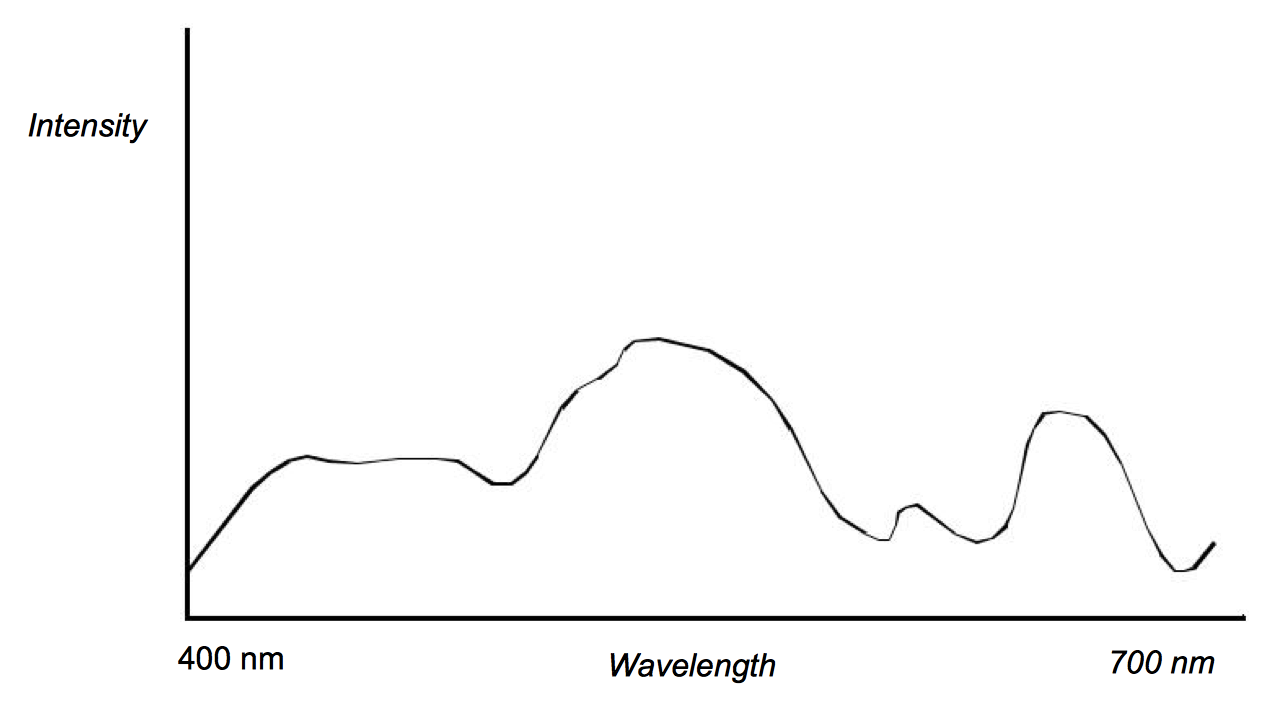
\includegraphics[width=0.8\textwidth]{Figure3-2}\\
  \caption{Wavelength versus Intensity plot.}\label{fig:Figure3-2}
\end{figure}

The two simplified component systems that we use to describe colors are RGB and HSV color systems. The RGB system represents colors based on their red, green, and blue intensities. This can be thought of as a three dimensional space with the axes being red, green, and blue. Some common colors and their RGB components are shown in Table \ref{table:Figure3-4}.

The HSV system represents colors based on their hue, saturation, and value. The value component is also known as the brightness or intensity component, and represents how much light is in the color. A value of 0.0 will always give you black and a value of 1.0 will give you something bright. The hue represents the dominant wavelength of the color and is often illustrated using a circle as in Figure \ref{fig:Figure3-5}. Each location on the circumference of this circle represents a different hue and can be specified using an angle. When we specify a hue we use the range from zero to one, where zero corresponds to zero degrees on the hue circle and one corresponds to 360 degrees. The saturation indicates how much of the hue is mixed into the color. For example, we can set the value to one, which gives us a bright color, and the hue to 0.66, to give us a dominant wavelength of blue. Now if we set the saturation to one, the color will be a bright primary blue. If we set the saturation to 0.5, the color will be sky blue, a blue with more white mixed in. If we set the saturation to zero, this indicates that there is no more of the dominant wavelength (hue) in the color than any other wavelength. As a result, the final color will be white (regardless of hue value). Table \ref{table:Figure3-4} lists HSV values for some common colors.

\begin{figure}[!htb]
  \centering
  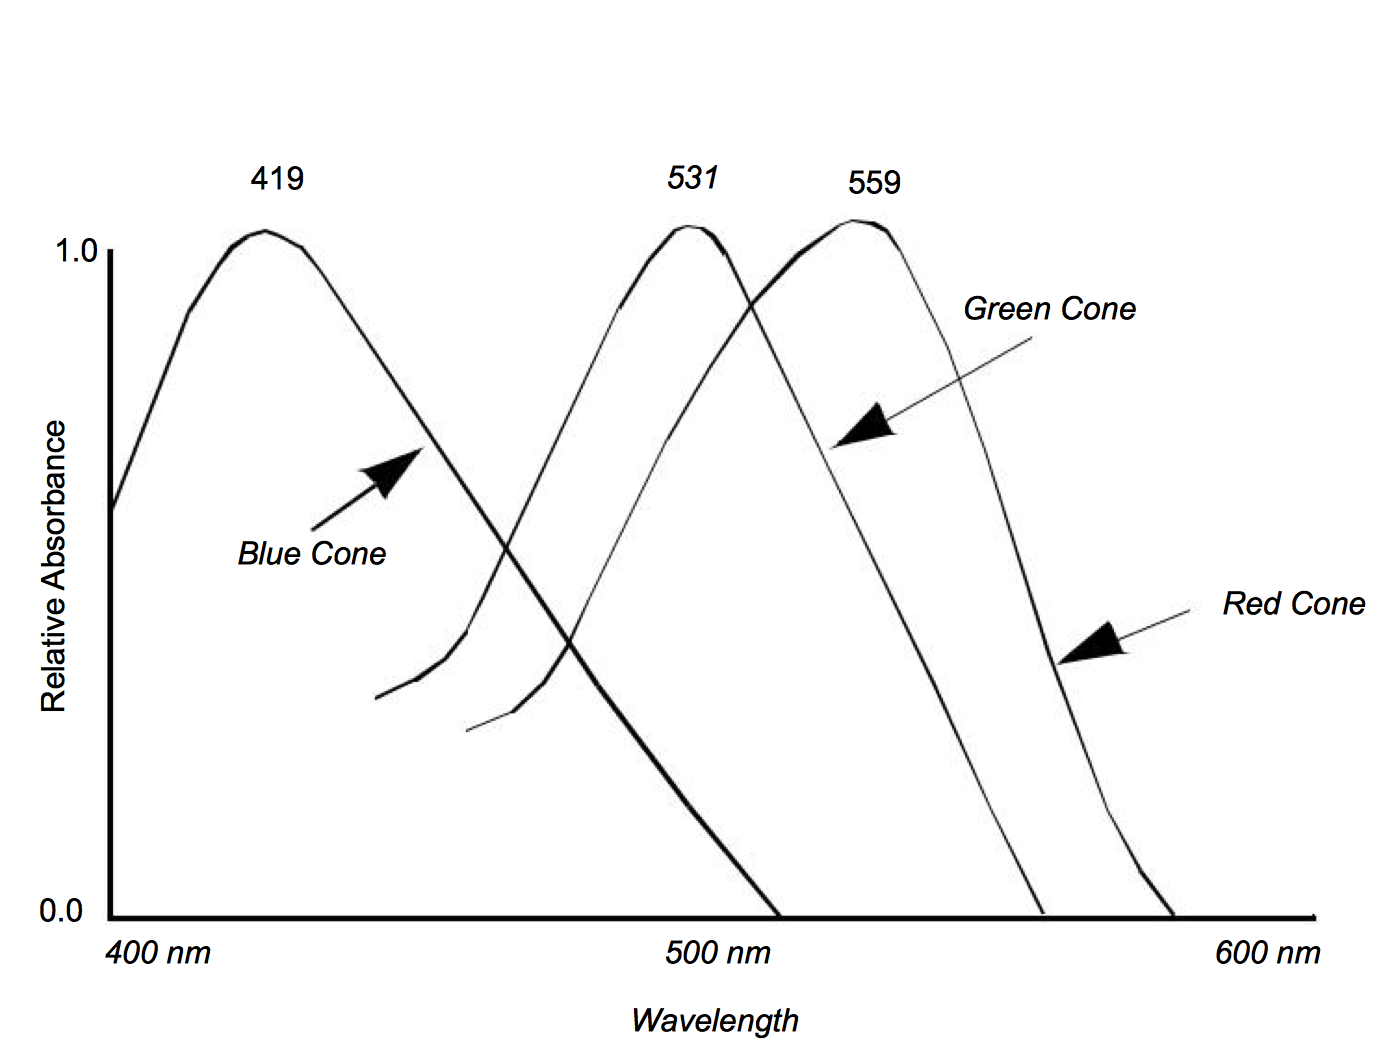
\includegraphics[width=0.8\textwidth]{Figure3-3}\\
  \caption{Relative absorbance of light by the three types of cones in the human retina.}\label{fig:Figure3-3}
\end{figure}

\begin{table}
	\centering
    \begin{tabular}{ | l | c | c | }
    \hline
    Color & RGB & HSV\\
    \hline
    Black & $0,0,0$ & $\ast,\ast,0$\\
    White & $1,1,1$ & $\ast,0,1$\\
    Red & $1,0,0$ & $0,1,1$\\
    Green & $0,1,0$ & $1/3,1,1$\\
    Blue & $0,0,1$ & $2/3,1,1$\\
    Cyan & $0,1,1$ & $1/2,1,1$\\
    Magenta & $1,0,1$ & $5/6,1,1$\\
    Yellow & $1,1,0$ & $1/6,1,1$\\
    Sky Blue & $1/2,1/2,1$ & $2/3,1/2,1$\\
    \hline
    \end{tabular}
    \caption{Common colors in RGB and HSV space}\label{table:Figure3-4}
\end{table}
  
\begin{figure}[!htb]
  \centering
  \begin{subfigure}[a]{0.6\textwidth}{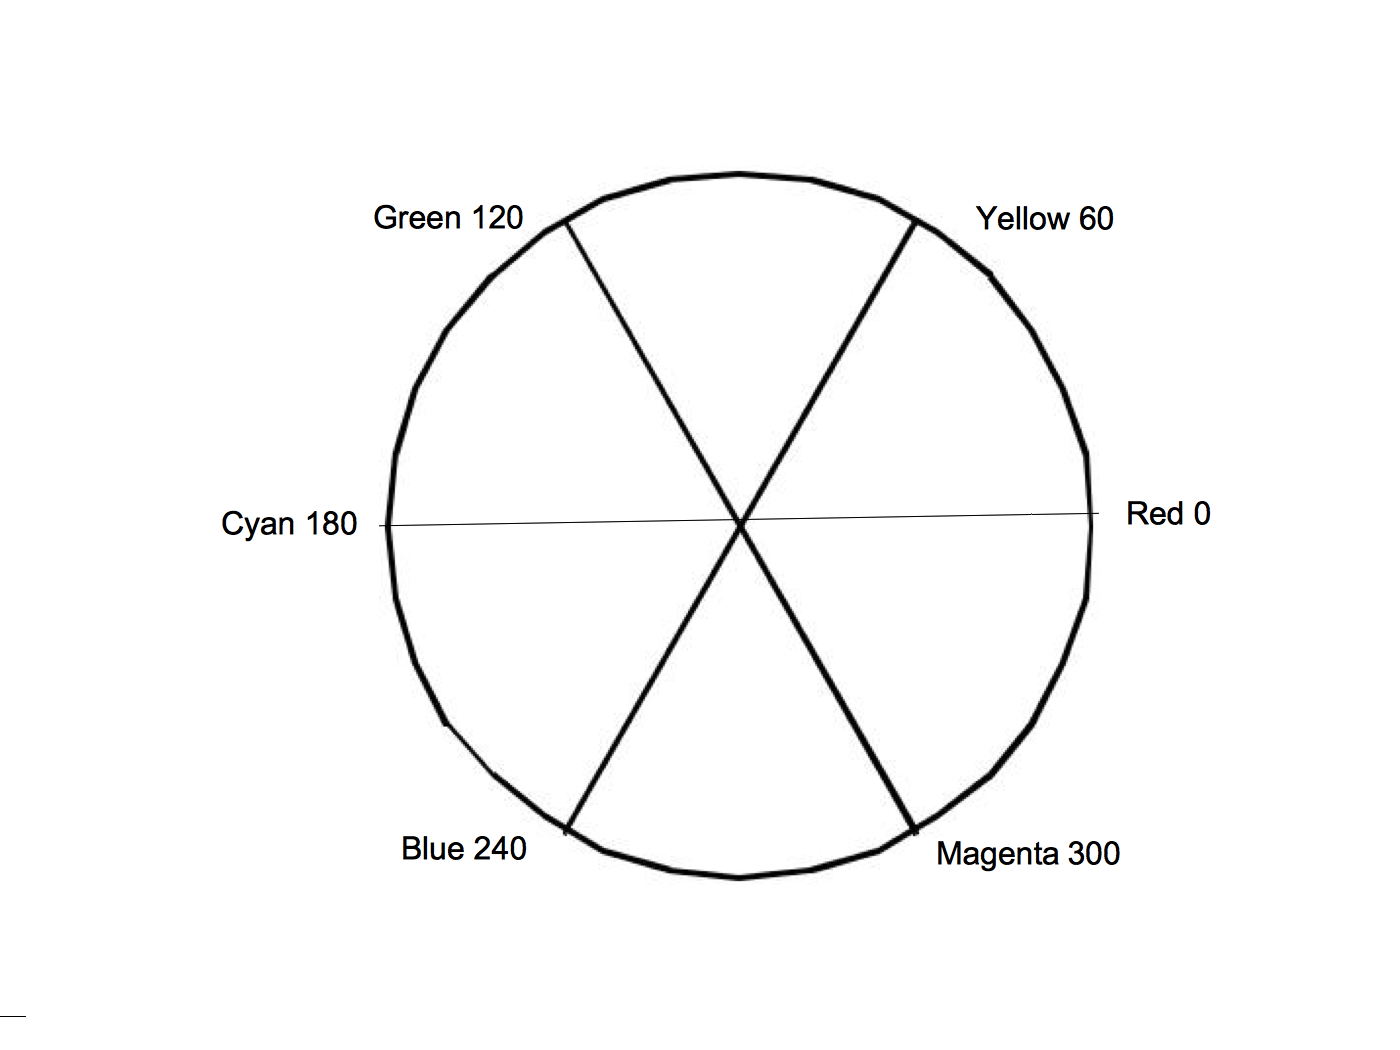
\includegraphics[width=\textwidth]{Figure3-5a}		  \label{fig:Figure3-5a}}
  \end{subfigure}
  \hfill
  \begin{subfigure}[b]{0.6\textwidth}{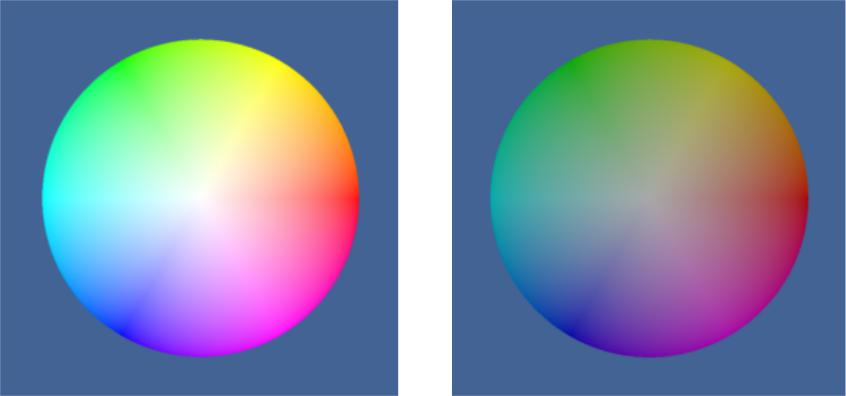
\includegraphics[width=\textwidth]{Figure3-5b}  	  \label{fig:Figure3-5b}}
  \end{subfigure}
  \caption{On the top, circular representation of hue. The other two
images on the bottom are slices through the HSV color space. The first slice
has a value of 1.0, the other has a value of 0.5.}
\label{fig:Figure3-5}
\end{figure}

\section{Lights}
\label{Lights}
One of the major factors controlling the rendering process is the interaction of light with the actors in the scene. If there are no lights, the resulting image will be black and rather uninformative. To a great extent it is the interaction between the emitted light and the surface (and in some cases the interior) of the actors in the scene that defines what we see. Once rays of light interact with the actors in a scene, we have something for our camera to view.

Of the many different types of lights used in computer graphics, we will discuss the simplest, the infinitely distant, point light source. This is a simplified model compared to the lights we use at home and work. The light sources that we are accustomed to typically radiate from a region in space (a filament in an incandescent bulb, or a light-emitting gas in a fluorescent light). The point source lighting model assumes that the light is emitted in all directions from a single point in space. For an infinite light source, we assume that it is positioned infinitely far away from what it is illuminating. This is significant because it implies that the incoming rays from such a source will be parallel to each other. The emissions of a local light source, such as a lamp in a room, are not parallel. Figure \ref{fig:Figure3-6} illustrates the differences between a local light source with a finite volume, versus an infinite point light source. The intensity of the light emitted by our infinite light sources also remains constant as it travels, in contrast to the actual $1/distance^2$ relationship physical lights obey. As you can see this is a great simplification, which later will allow us to use less complex lighting equations.

\begin{figure}[!htb]
  \centering
  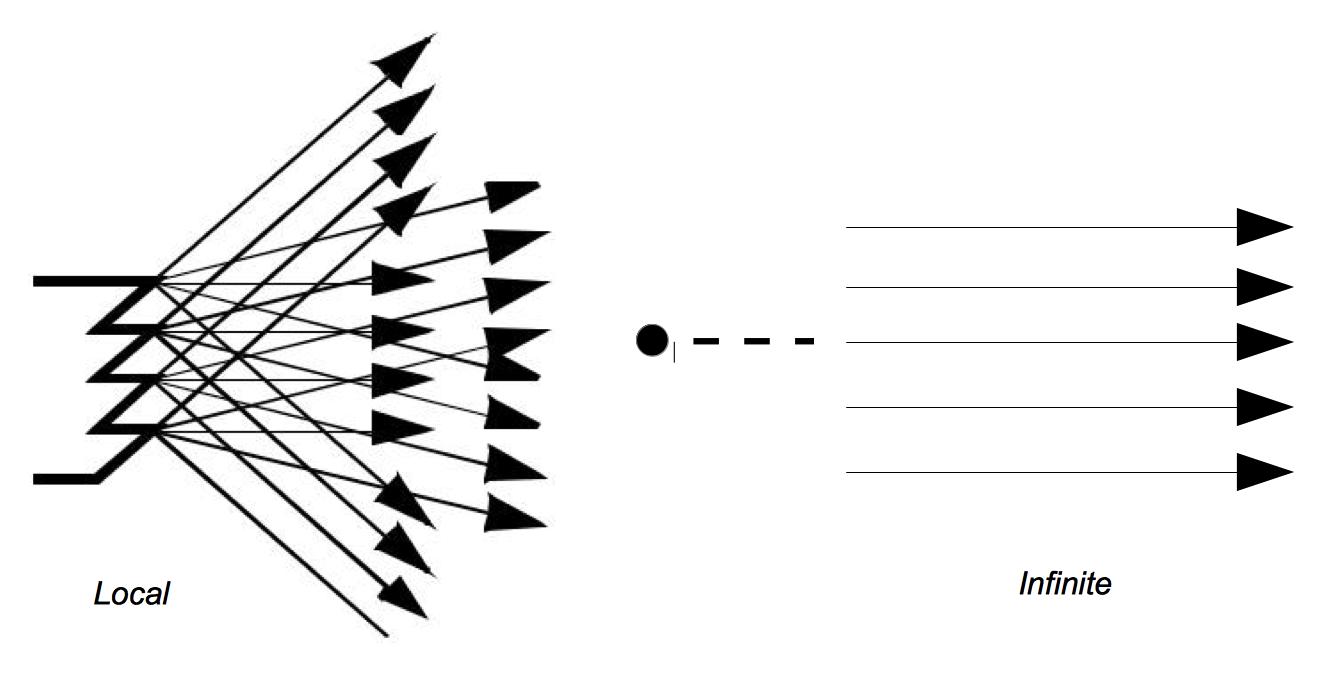
\includegraphics[width=0.8\textwidth]{Figure3-6}\\
  \caption{Local light source with a finite volume versus an infinite point light source.}\label{fig:Figure3-6}
\end{figure}

\section{Surface Properties}
As rays of light travel through space, some of them intersect our actors. When this happens, the rays of light interact with the surface of the actor to produce a color. Part of this resulting color is actually not due to direct light, but rather from \emph{ambient} light that is being reflected or scattered from other objects. An ambient lighting model accounts for this and is a simple approximation of the complex scattering of light that occurs in the real world. It applies the intensity curve of the light source to the color of the object, also expressed as an intensity curve. The result is the color of the light we see when we look at that object. With such a model, it is important to realize that a white light shining on a blue ball is indistinguishable from a blue light shining on a white ball. The ambient lighting equation is

\begin{equation}\label{eq:3.1}
  R_a = L_c \cdot O_a
\end{equation}

where $R_a$ is the resulting intensity curve due to ambient lighting, $L_c$ is the intensity curve of the ambient light, and $O_a$ is the color curve of the object. To help keep the equations simple we assume that all of the direction vectors are normalized (i.e., have a magnitude of one).

Two components of the resulting color depend on direct lighting. \emph{Diffuse lighting}, which is also known as Lambertian reflection, takes into account the angle of incidence of the light onto an object. Figure \ref{fig:Figure3-7} shows the image of a cylinder that becomes darker as you move laterally from its center. The cylinder's color is constant; the amount of light hitting the surface of the cylinder changes. At the center, where the incoming light is nearly perpendicular to the surface of the cylinder, it receives more rays of light per surface area. As we move towards the side, this drops until finally the incoming light is parallel to the side of the cylinder and the resulting intensity is zero.

\begin{figure}[!htb]
  \centering
  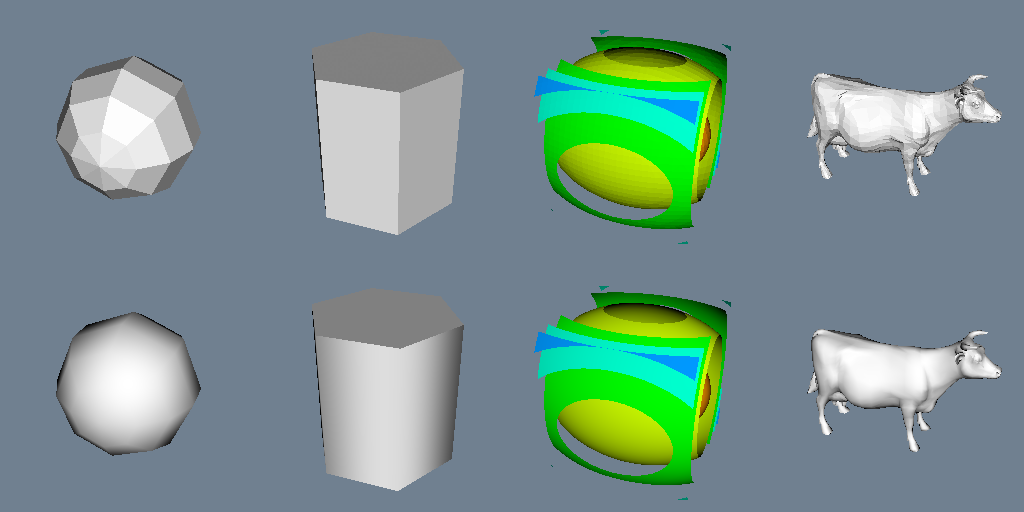
\includegraphics[width=0.8\textwidth]{Figure3-7}\\
  \caption{Flat and Gouraud shading. Different shading methods can dramatically improve the look of an object represented with polygons. On the top, flat shading uses a constant surface normal across each polygon. On the bottom, Gouraud shading interpolates normals from polygon vertices to give a smoother look.}\label{fig:Figure3-7}
\end{figure}

The contribution from diffuse lighting is expressed in Equation \ref{eq:3.2} and illustrated in Figure \ref{fig:Figure3-8}.

\begin{equation}\label{eq:3.2}
  R_d = L_cO_d[\overrightarrow{O}_n \cdot (-\overrightarrow{L}_n)]
\end{equation}

where $R_d$ is the resulting intensity curve due to diffuse lighting, $L_c$ is the intensity curve for the light, and $O_c$ is the color curve for the object. Notice that the diffuse light is a function of the relative angle between incident light vector and $\overrightarrow{L}_n$ and the surface normal of the object $\overrightarrow{O}_n$. As a result diffuse lighting is independent of viewer position.

\emph{Specular} lighting represents direct reflections of a light source off a shiny object. Figure \ref{fig:Figure3-10} shows a diffusely lit ball with varying specular reflection. The specular intensity (which varies between the top and bottom rows) controls the intensity of the specular lighting. The specular power, $O_sp$, indicates how shiny an object is, more specifically it indicates how quickly specular reflections diminish as the reflection angles deviate from a perfect reflection. Higher values indicate a faster drop off, and therefore a shinier surface. Referring to Figure \ref{fig:Figure3-9}, the equation for specular lighting is

\begin{equation}\label{eq:3.3}
  R_s . = L_cO_s[\overrightarrow{S} \cdot (-\overrightarrow{C}_n)] ^{O_{sp}}\\
\overrightarrow{S} = 2[\overrightarrow{O}_n \cdot (-\overrightarrow{L}_n)]\overrightarrow{O}_n + \overrightarrow{L}_n
\end{equation}
where $\overrightarrow{C}_n$ is the direction of projection for the camera and $\overrightarrow{S}$ is the direction of specular reflection.

\begin{figure}[!htb]
  \centering
  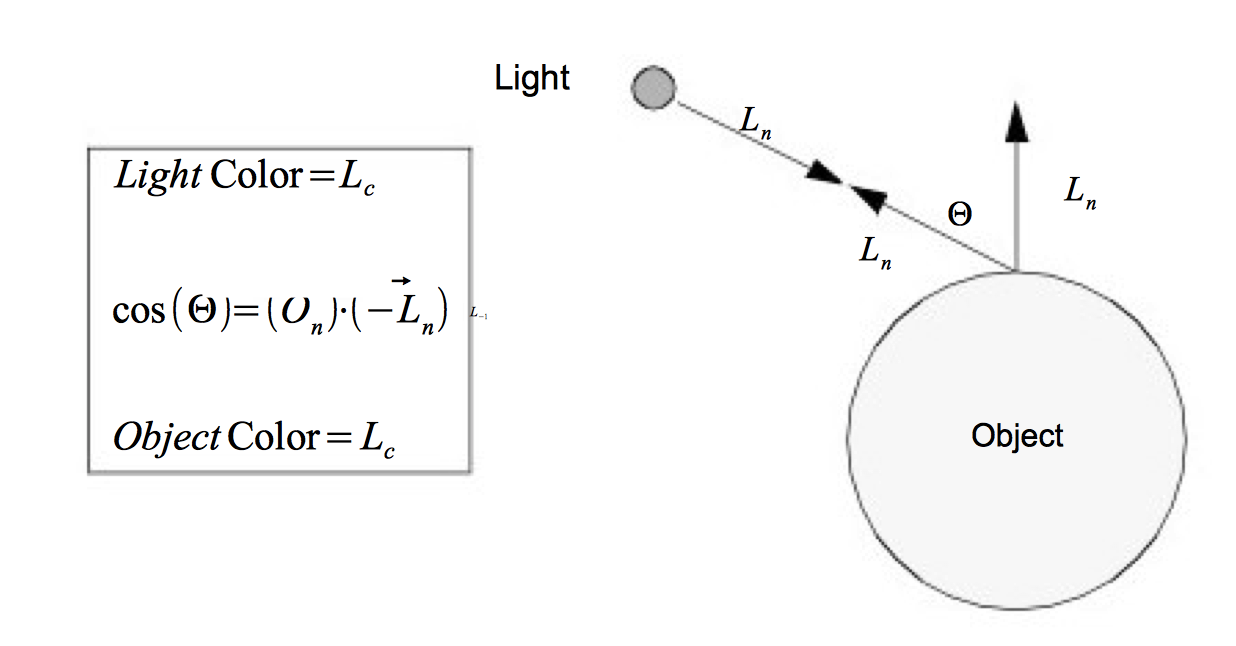
\includegraphics[width=0.8\textwidth]{Figure3-8}\\
  \caption{Diffuse lighting}\label{fig:Figure3-8}
\end{figure}

\begin{figure}[!htb]
  \centering
  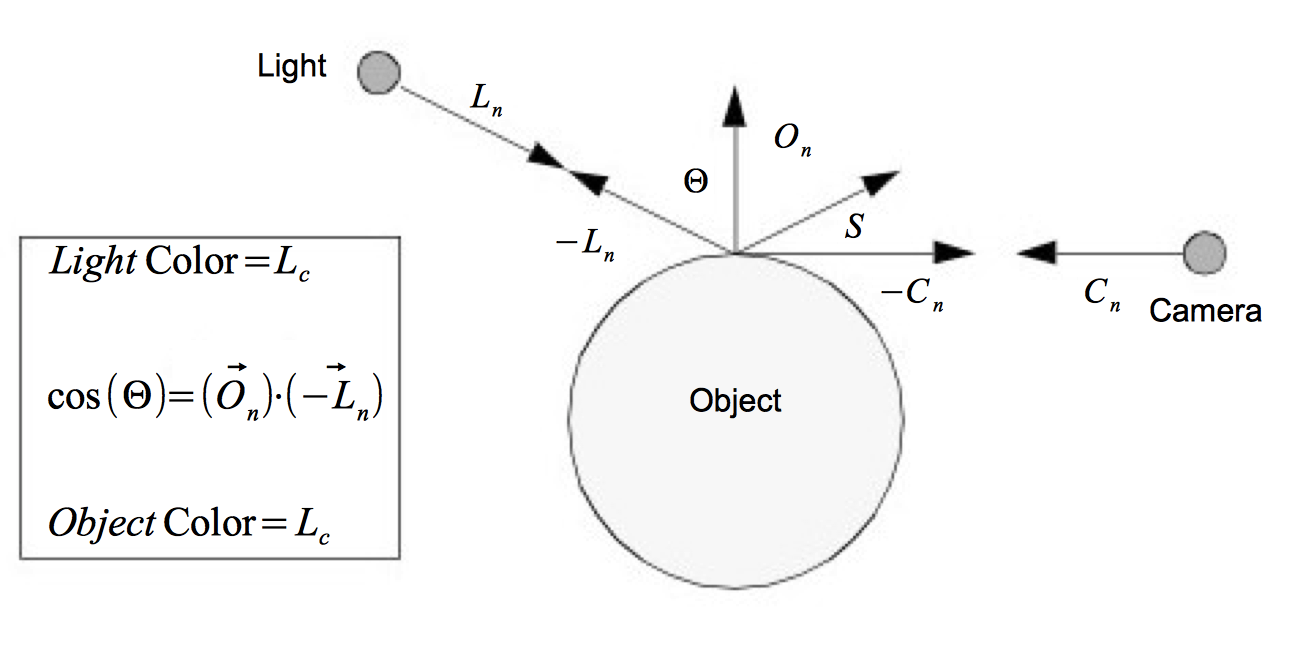
\includegraphics[width=0.8\textwidth]{Figure3-9}\\
  \caption{Specular lighting.}\label{fig:Figure3-9}
\end{figure}

We have presented the equations for the different lighting models independently. We can apply all lighting models simultaneously or in combination. Equation \ref{eq:3.4} combines ambient, diffuse and specular lighting into one equation.

\begin{equation}\label{eq:3.4}
  R_c = O_{ai}O_{ac}L_c - O_{di}O_{dc}L_c(\overrightarrow{O}_n \cdot \overrightarrow{L}_n) + O_{si}O_{sc}L_c[\overrightarrow{S} \cdot(-\overrightarrow{C}_n)]^{O_{sp}}
\end{equation}

The result is a color at a point on the surface of the object. The constants $O_{ai}$, $O_{di}$, and $O_{si}$ control the relative amounts of ambient, diffuse and specular lighting for an object. The constants $O_{ac}$ $O_{dc}$ and $O_{sc}$ specify the colors to be used for each type of lighting. These six constants along with the specular power are part of the surface material properties. (Other properties such as transparency will be covered in later sections of the text.) Different combinations of these property values can simulate dull plastic and polished metal. The equation assumes an infinite point light source as described in “Lights” on \ref{Lights}. However the equation can be easily modified to incorporate other types of directional lighting.

\begin{figure}[!htb]
  \centering
  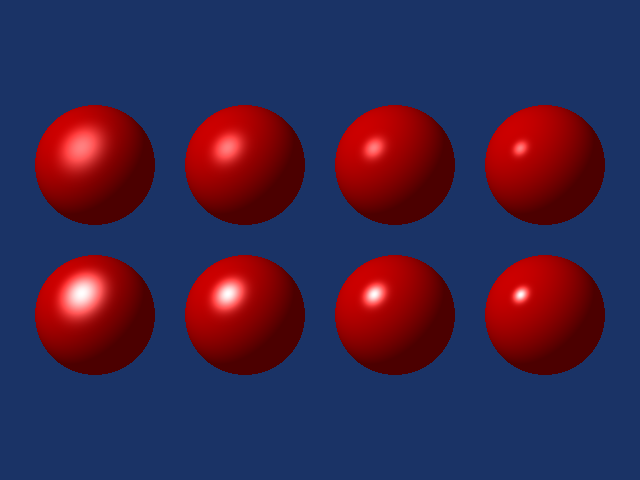
\includegraphics[width=0.8\textwidth]{Figure3-10}\\
  \caption{Effects of specular coefficients. Specular coefficients control the apparent "shininess" of objects. The top row has a specular intensity value of 0.5; the bottom row 1.0. Along the horizontal direction the specular power changes. The values (from left to right) are 5, 10, 20, and 40.}\label{fig:Figure3-10}
\end{figure}

\section{Cameras}

We have light sources that are emitting rays of light and actors with surface properties. At every point on the surface of our actors this interaction results in some composite color (i.e., combined color from light, object surface, specular, and ambient effects). All we need now to render the scene is a camera. There are a number of important factors that determine how a 3D scene gets projected onto a plane to form a 2D image (see Figure \ref{fig:Figure3-11}). These are the position, orientation, and focal point of the camera, the method of camera projection , and the location of the camera clipping planes.

\begin{figure}[!htb]
  \centering
  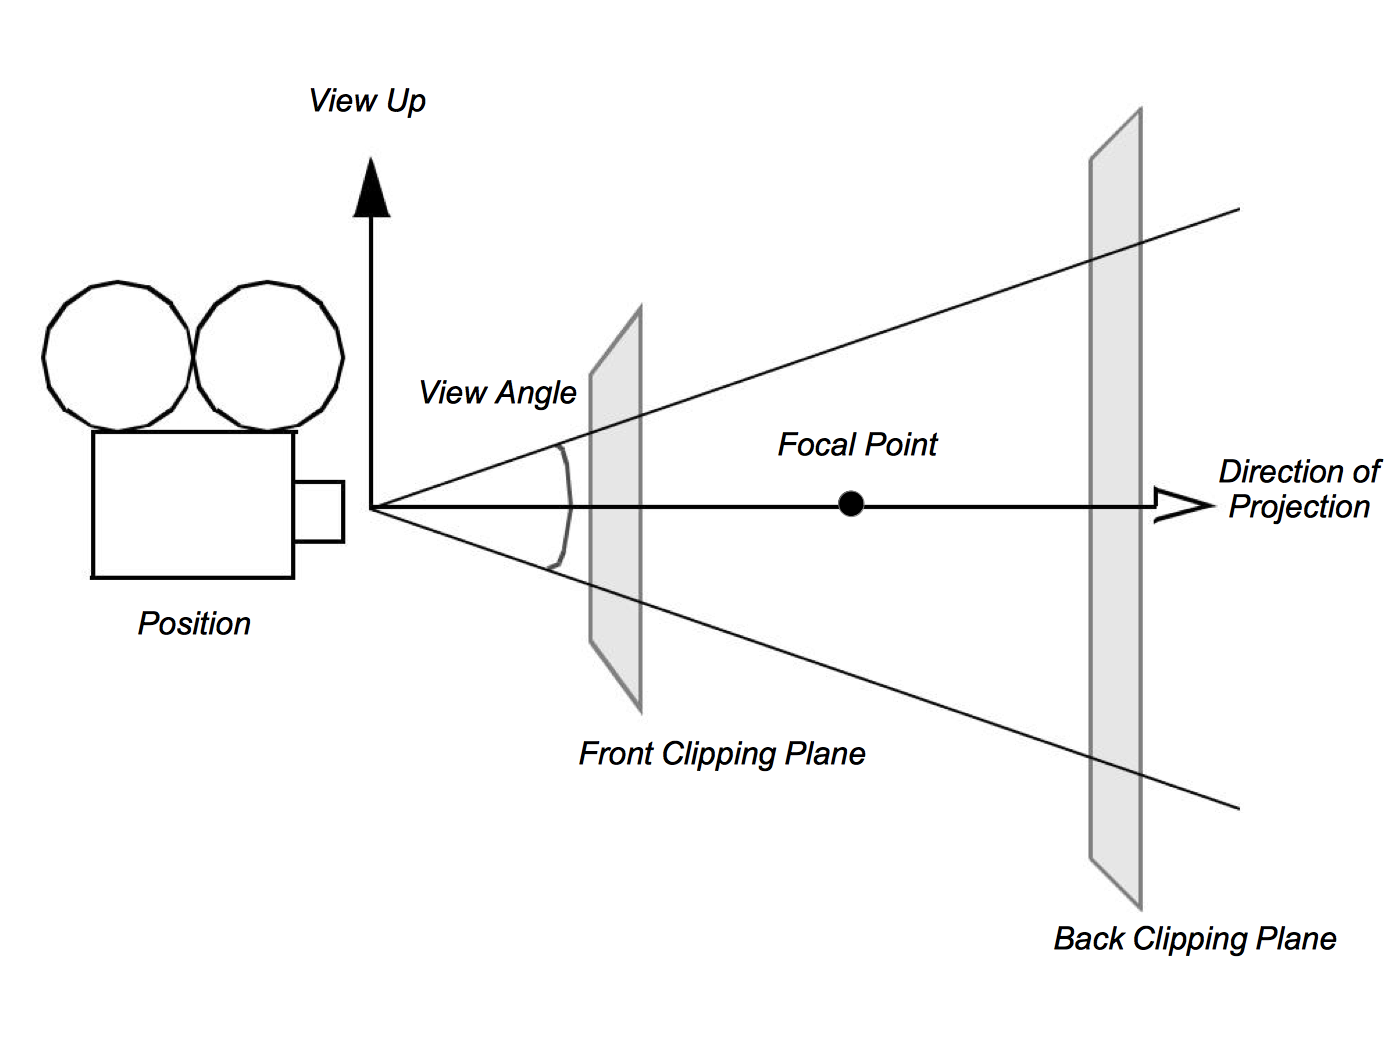
\includegraphics[width=0.8\textwidth]{Figure3-11}\\
  \caption{Camera attributes.}\label{fig:Figure3-11}
\end{figure}

The position and focal point of the camera define the location of the camera and where it points. The vector defined from the camera position to the focal point is called the direction of projection . The camera image plane is located at the focal point and is typically perpendicular to the projection vector. The camera orientation is controlled by the position and focal point plus the camera view-up vector. Together these completely define the camera view. 

The method of projection controls how the actors are mapped to the image plane. \emph{Orthographic projection} is a parallel mapping process. In orthographic projection (or parallel projection) all rays of light entering the camera are parallel to the projection vector. \emph{Perspective projection} occurs when all light rays go through a common point (i.e., the viewpoint or center of projection). To apply perspective projection we must specify a perspective angle or camera view angle.

The front and back clipping planes intersect the projection vector, and are usually perpendicular to it. The clipping planes are used to eliminate data either too close to the camera or too far away. As a result only actors or portions of actors within the clipping planes are (potentially) visible. Clipping planes are typically perpendicular to the direction of projection. Their locations can be set using the camera’s clipping range. The location of the planes are measured from the camera’s position along the direction of projection. The front clipping plane is at the minimum range value, and the back clipping plane is at the maximum range value. Later on in Chapter 7 , when we discuss stereo rendering, we will see examples of clipping planes that are not perpendicular to the direction of projection.

Taken together these camera parameters define a rectangular pyramid, with its apex at the camera’s position and extending along the direction of projection. The pyramid is truncated at the top with the front clipping plane and at the bottom by the back clipping plane. The resulting view frustum defines the region of 3D space visible to the camera.

While a camera can be manipulated by directly setting the attributes mentioned above, there are some common operations that make the job easier. Figure \ref{fig:Figure3-12} and Figure \ref{fig:Figure3-13} will help illustrate these operations. Changing the azimuth of a camera rotates its position around its view up vector, centered at the focal point . Think of this as moving the camera to the left or right while always keeping the distance to the focal point constant. Changing a camera’s elevation rotates its position around the cross product of its direction of projection and view up centered at the focal point. This corresponds to moving the camera up and down. To roll the camera, we rotate the view up vector about the view plane normal. Roll is sometimes called twist.

The next two motions keep the camera’s position constant and instead modify the focal point. Changing the yaw rotates the focal point about the view up centered at the camera’s position. This is like an azimuth, except that the focal point moves instead of the position. Changes in pitch rotate the focal point about the cross product of the direction of projection and view up centered at the camera’s position. Dollying in and out moves the camera’s position along the direction of projection, either closer or farther from the focal point. This operation is specified as the ratio of its current distance to its new distance. A value greater than one will dolly in, while a value less than one will dolly out. Finally, zooming changes the camera’s view angle, so that more or less of the scene falls within the view frustum.

\begin{figure}[!htb]
  \centering
  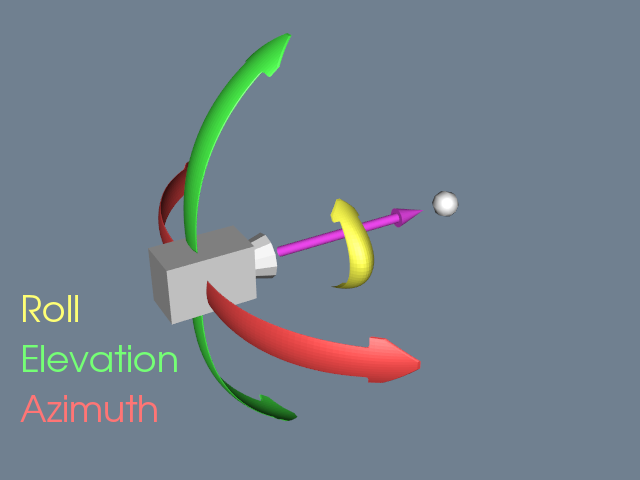
\includegraphics[width=0.8\textwidth]{Figure3-12}\\
  \caption{Camera movements around the focal point.}\label{fig:Figure3-12}
\end{figure}

\begin{figure}[!htb]
  \centering
  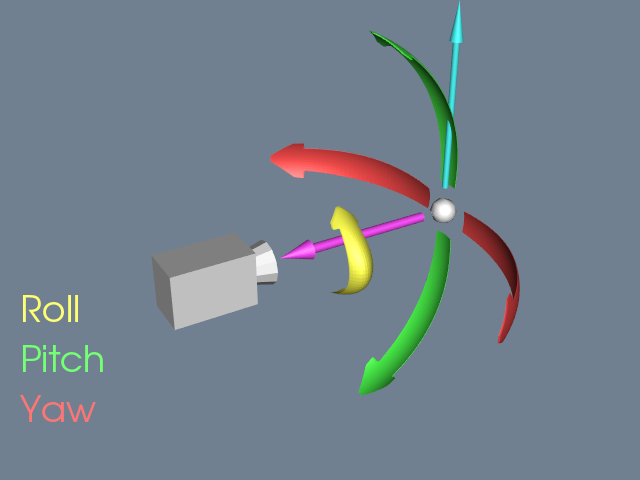
\includegraphics[width=0.8\textwidth]{Figure3-13}\\
  \caption{Camera movements around the camera position.}\label{fig:Figure3-13}
\end{figure}

Once we have the camera situated, we can generate our 2D image. Some of the rays of light traveling through our 3D space will pass through the lens on the camera. These rays then strike a flat surface to produce an image. This effectively projects our 3D scene into a 2D image. The camera’s position and other properties determine which rays of light get captured and projected. More specifically, only rays of light that intersect the camera’s position, and are within its viewing frustum, will affect the resulting 2D image.

This concludes our brief rendering overview. The light has traveled from its sources to the actors, where it is reflected and scattered. Some of this light gets captured by the camera and produces a 2D image. Now we will look at some of the details of this process.

\section{Coordinate Systems}

There are four coordinate systems commonly used in computer graphics and two different ways of representing points within them (Figure \ref{fig:Figure3-14}). While this may seem excessive, each one serves a purpose. The four coordinate systems we use are: \emph{model}, \emph{world} , \emph{view}, and \emph{display}.

The model coordinate system is the coordinate system in which the model is defined, typically a local Cartesian coordinate system. If one of our actors represents a football, it will be based on a coordinate system natural to the football geometry (e.g., a cylindrical system). This model has an inherent coordinate system determined by the decisions of whoever generated it. They may have used inches or meters as their units, and the football may have been modelled with any arbitrary axis as its major axis.

The world coordinate system is the 3D space in which the actors are positioned. One of the actor’s responsibilities is to convert from the model’s coordinates into world coordinates. Each model may have its own coordinate system but there is only one world coordinate system. Each actor must scale, rotate, and translate its model into the world coordinate system. (It may also be necessary for the modeller to transform from its natural coordinate system into a local Cartesian system. This is because actors typically assume that the model coordinate system is a local Cartesian system.) The world coordinate system is also the system in which the position and orientation of cameras and lights are specified.

The view coordinate system represents what is visible to the camera. This consists of a pair of x and y values, ranging between (-1,1), and a z depth coordinate. The x, y values specify location in the image plane, while the z coordinate represents the distance, or range, from the camera. The camera’s properties are represented by a four by four transformation matrix (to be described shortly), which is used to convert from world coordinates into view coordinates. This is where the perspective effects of a camera are introduced.

The display coordinate system uses the same basis as the view coordinate system, but instead of using negative one to one as the range, the coordinates are actual x, y pixel locations on the image plane. Factors such as the window’s size on the display determine how the view coordinate range of (-1,1) is mapped into pixel locations. This is also where the viewport comes into effect.

\begin{figure}[!htb]
  \centering
  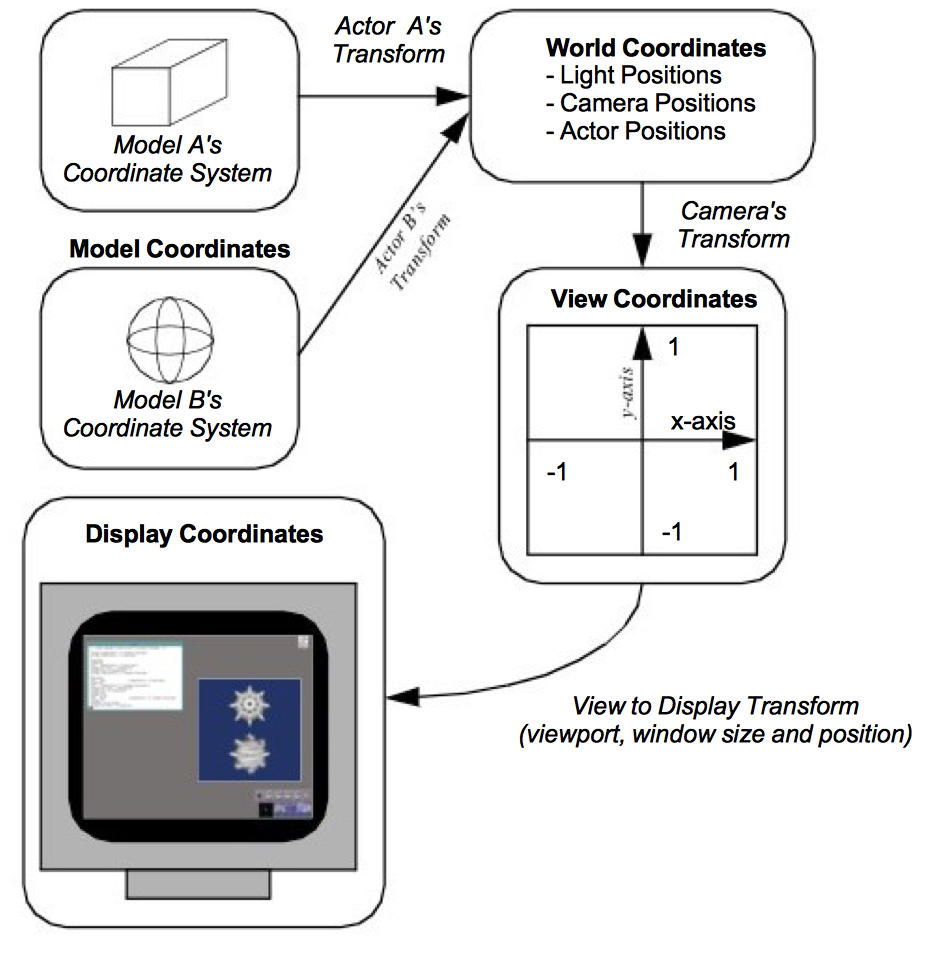
\includegraphics[width=0.8\textwidth]{Figure3-14}\\
  \caption{ Modelling, world, view and display coordinate system.}\label{fig:Figure3-14}
\end{figure}

You may want to render two different scenes, but display them in the same window. This can be done by dividing the window into rectangular viewports. Then, each renderer can be told what portion of the window it should use for rendering. The viewport ranges from (0,1) in both the x and y axis. Similar to the view coordinate system, the z-value in the display coordinate system also represents depth into the window. The meaning of this z-value will be further described in the section titled “Z-Buffer” on page \pageref{Z-Buffer}.


\section{Coordinate Transformation}

When we create images with computer graphics, we project objects defined in three dimensions onto a two-dimensional image plane. As we saw earlier, this projection naturally includes perspective. To include projection effects such as vanishing points we use a special coordinate system called homogeneous coordinates.

The usual way of representing a point in 3D is the three element Cartesian vector $(x, y, z)$. Homogeneous coordinates are represented by a four element vector $( x_hh, y_h, z_h, w_h )$. The conversion between Cartesian coordinates and homogeneous coordinates is given by:

\begin{equation}\label{eq:3.5}
x = \frac{x_h}{w_h}\ \ \ \  x = \frac{y_h}{w_h}\ \ \ \ x = \frac{z_h}{w_h}
\end{equation}

Using homogeneous coordinates we can represent an infinite point by setting w h to zero. This capability is used by the camera for perspective transformations. The transformations are applied by using a 4x4 transformation matrix . Transformation matrices are widely used in computer graphics because they allow us to perform translation, scaling, and rotation of objects by repeated matrix multiplication. Not all of these operations can be performed using a 3x3 matrix.

For example, suppose we wanted to create a transformation matrix that translates a point $( x, y, z)$ in Cartesian space by the vector $( t_x , t_y, t_z)$. We need only construct the translation matrix given by

\begin{equation}\label{eq:3.6}
T_T = \left[\begin{array}{cccc}
1 & 0 & 0 & t_x       \\
0 & 1 & 0 & t_y      \\
0 & 0 & 1 & t_z      \\
0 & 0 & 0 & 1
\end{array}\right]
\end{equation}

and then postmultiply it with the homogeneous coordinate $(x_h, y_h, z_h, w_h)$. To carry this example through, we construct the homogeneous coordinate from the Cartesian coordinate $( x, y, z)$ by setting $w_h = 1$ to yield $(x, y, z, 1)$. Then to determine the translated point $(x' , y', z')$ we premultiply current position by the transformation matrix $T_T$ to yield the translated coordinate. Substituting into Equation \ref{eq:3.6} we have the result

\begin{equation}\label{eq:3.7}
\left[\begin{array}{c}
x'      \\
y'       \\
z'      \\
w'
\end{array}\right] =\left[\begin{array}{cccc}
1 & 0 & 0 & t_x       \\
0 & 1 & 0 & t_y       \\
0 & 0 & 1 & 0      \\
0 & 0 & 0 & 1
\end{array}\right] \cdot
\left[\begin{array}{c}
x      \\
y       \\
z      \\
1
\end{array}\right] 
\end{equation}

Converting back to Cartesian coordinates via Equation\ref{eq:3.5} we have the expected solution

\begin{equation}\label{eq:3.8}
x' = x +t_x \\
y' = y + t_y \\
z' = z + t_z
\end{equation}

The same procedure is used to scale or rotate an object. To scale an object we use the transformation matrix

\begin{equation}\label{eq:3.9}
T_s = \left[\begin{array}{cccc}
s_x & 0 & 0 & 0 \\
0 & s_y & 0 & 0 \\
0 & 0 & s_z & 0 \\
0 & 0 & 0 & 1
\end{array}\right]
\end{equation}

where the parameters $s_x, s_y$, and $s_z$ are scale factors along the $x, y, z$ axes. Similarly we can rotate an object around the $x$ axes by angle $\theta$ using the matrix

\begin{equation}\label{eq:3.10}
T_{R_x} = \left[\begin{array}{cccc}
1 & 0 & 0 & 0 \\
0 & \cos\theta & -\sin\theta & 0 \\
0 & \sin\theta & \cos\theta & 0 \\
0 & 0 & 0 & 1
\end{array}\right]
\end{equation}

Around the $y$ axis we use

\begin{equation}\label{eq:3.11}
TT_{R_y} = \left[\begin{array}{cccc}
\cos\theta & 0 & \sin\theta0 & 0 \\
0 & 1 & 0 & 0 \\
-\sin\theta & 0 & \cos\theta & 0 \\
0 & 0 & 0 & 1
\end{array}\right]
\end{equation}

and around the $z$ axis we use

\begin{equation}\label{eq:3.12}
T_{R_z} = \left[\begin{array}{cccc}
\cos\theta & -\sin\theta & 0 & 0 \\
\sin\theta & \cos\theta & 0 & 0 \\
0 & 0 & 0 & 0 \\
0 & 0 & 0 & 1
\end{array}\right]
\end{equation}

Another useful rotation matrix is used to transform one coordinate axes $x-y-z$ to another coordinate axes $x'-y'-z'$. To derive the transformation matrix we assume that the unit $x'$. To derive the transformation matrix we assume that the unit $x'$ axis make the angles $(\theta_{x'x},\theta_{x'y},\theta_{x'z})$ around the x-y-z axes (these are called direction cosines). Similarly, the unit $y'$ axis makes the angles $(\theta_{y'x},\theta_{y'y},\theta_{y'z})$ and the unit $z'$ axis makes the angles $(\theta_{z'x},\theta_{z'y},\theta_{z'z})$. The resulting rotation matrix is formed by placing the direction cosines along the rows of the transformation matrix as follows

\begin{equation}\label{eq:3.137}
T_R = \left[\begin{array}{cccc}
\cos\theta_{x'x} & \cos\theta_{x'y} & \cos\theta_{x'z} & 0 \\
\cos\theta_{y'x} & \cos\theta_{z'y} & \cos\theta_{y'z} & 0 \\
\cos\theta_{z'x} & \cos\theta_{z'y} & \cos\theta_{z'z} & 0 \\
0 & 0 & 0 & 1
\end{array}\right]
\end{equation}

Rotations occur about the coordinate origin. It is often more convenient to rotate around the center of the object (or a user-specified point). Assume that we call this point the object’s center . To rotate around we Oc must first translate the object to the Oorigin, apply rotations, and then translate the object back.

Transformation matrices can be combined by matrix multiplication to achieve combinations of translation, rotation, and scaling. It is possible for a single transformation matrix to represent all types of transformation simultaneously. This matrix is the result of repeated matrix multiplications. A word of warning: The order of the multiplication is important. For example, multiplying a translation matrix by a rotation matrix will not yield the same result as multiplying the rotation matrix by the translation matrix.

\section{Actor Geometry}

\subsection*{Modelling}

\subsection*{Actor Location and Orientation}

\section{Graphics Hardware}

\subsection*{Raster Devices}

\subsection*{Interfacing to the Hardware}

\subsection*{Rasterization}

\subsection*{Z-Buffer}

\label{Z-Buffer}

\section{Putting It All Together}

\section{Chapter Summary}

Rendering is the process of generating an image using a computer. Computer graphics is the field of study that encompasses rendering techniques, and forms the foundation of data visualization.

Three-dimensional rendering techniques simulate the interaction of lights and cameras with objects, or actors, to generate images. A scene consists of a combination of lights, cameras, and actors. Object-order rendering techniques generate images by rendering actors in a scene in order. Image-order techniques render the image one pixel at a time. Polygon based graphics hardware is based on object-order techniques. Ray tracing or ray-casting is an image-order technique.

Lighting models require a specification of color. We saw both the RGB (red-green-blue) and HSV (hue-saturation-value) color models. The HSV model is a more natural model than the RGB model for most users. Lighting models also include effects due to ambient, diffuse, and specular lighting.

There are four important coordinate systems in computer graphics. The model system is the 3D coordinate system where our geometry is defined. The world system is the global Cartesian system. All modelled data is eventually transformed into the world system. The view coordinate system represents what is visible to the camera. It is a 2D system scaled from (-1,1). The display coordinate system uses actual pixel locations on the computer display.

Homogeneous coordinates are a 4D coordinate system in which we can include the effects of perspective transformation. Transformation matrices are \(4 \times 4\) matrices that operate on homogeneous coordinates. Transformation matrices can represent the effects of translation, scaling, and rotation of an actor. These matrices can be multiplied together to give combined transformations.

Graphics programming is usually implemented using higher-level graphics libraries and specialized hardware systems. These dedicated systems offer better performance and easier implementation of graphics applications. Common techniques implemented in these systems include dithering and z-buffering. Dithering is a technique to simulate colors by mixing combinations of available colors. Z-buffering is a technique to perform hidden-line and hidden-surface removal.

\section{Bibliographic Notes}
\label{Ch03BibNotes}
This chapter provides the reader with enough information to understand the basic issues and terms used in computer graphics. There are a number of good text books that cover computer graphics in more detail and are recommended to readers who would like a more thorough understanding. The bible of computer graphics is \cite{FoleyVanDam90}. For those wishing for less intimidating books \cite{BurgerGillies89} and \cite{Watt93} are also useful references. You also may wish to peruse proceedings of the ACM SIGGRAPH conferences. These include papers and references to other papers for some of the most important work in computer graphics. \cite{Carlson85} provides a good introduction for those who wish to learn more about the human vision system.


\printbibliography
